\documentclass[a4paper,11pt]{article}

%Headers
\usepackage[dvips]{graphicx}    %package that does pdfs
\usepackage{color}              %this needs to be here also
\usepackage{ulem}
\usepackage{amsmath}
\usepackage{pgfplots}
\usepackage{adjustbox}
\usepackage{graphicx}
\usepackage{enumitem}
\usepackage{listings}
\usepackage{tikz}

\newcommand*\circled[1]{\tikz[baseline=(char.base)]{
             \node[shape=circle,draw,inner sep=2pt] (char) {#1};}}
\newcommand{\mybf}[1]{\boldsymbol{#1}}
\newcommand{\norm}[1]{\lvert\lvert #1 \rvert\rvert}

\title{%
	Problem Set 3\\
	\large MIT CW Linear Algebra (18.06)
}
\author{Aviel Livay}
\date{\today}

\begin{document}
\maketitle


\section*{Section 3.2}
\subsection*{Problem 13 (former problem 18)} 
\begin{align}
\begin{bmatrix}
x \\
y \\
z \\
\end{bmatrix}
=
\begin{bmatrix}
12 \\
0 \\
0 \\
\end{bmatrix}
+y
\begin{bmatrix}
3 \\
1 \\
0 \\
\end{bmatrix}
+z
\begin{bmatrix}
1 \\
0 \\
1 \\
\end{bmatrix}
\end{align}
\subsection*{Problem 18 (former problem 24)} 
I don't know.
\subsection*{Problem 30 (former problem 36)} 
This was my wrong solution: if $A$ has a rank of $r$. That means that the null space of $A$ can be represented as a linear combination of $n-r$ vectors. Any additional row that is contributed by $B$ can be either dependent on the previous rows or not and thus either leaves the rank at $r$ or increase it to $r+1$ which means that the sub space looses one degree of freedom. So $N(C) \subset N(A)$\\
The correct solution is that the null space of A should take 
\begin{align}
\begin{bmatrix}
A  \\
B  \\
\end{bmatrix} 
\begin{bmatrix}
\mybf{x_1}  \\
\mybf{x_2}  \\
\end{bmatrix}
= \mybf{0}
\end{align}
so both $A\mybf{x_1}$ AND $B\mybf{x_2}$ should equal 0 and $N(C) = N(A)  \cap N(B)$
\subsection*{Problem 32 (former problem 37)} 
\begin{align}
\begin{bmatrix}
-1 & 0  & 1  & -1 & 0  & 0  \\
1  & -1 & 0  & 0  & -1 & 0  \\
0  & 1  & -1 & 0  & 0  & -1 \\
0  & 0  & 0  & 1  & 1  & 1  \\
\end{bmatrix}
\end{align}
\begin{align}
\begin{bmatrix}
-1 & 0  & 1  & -1 & 0  & 0  \\
0  & -1 & 1  & -1 & -1 & 0  \\
0  & 1  & -1 & 0  & 0  & -1 \\
0  & 0  & 0  & 1  & 1  & 1  \\
\end{bmatrix}
\end{align}
\begin{align}
\begin{bmatrix}
-1 & 0  & 1  & -1 & 0  & 0  \\
0  & -1 & 1  & -1 & -1 & 0  \\
0  & 0  & 0  & -1 & -1 & -1 \\
0  & 0  & 0  & 1  & 1  & 1  \\
\end{bmatrix}
\end{align}
\begin{align}
\begin{bmatrix}
\circled{-1} &           0  & 1  &           -1 &  0 &  0 \\
0            & \circled{-1} & 1  &           -1 & -1 &  0 \\
0            &           0  & 0  & \circled{-1} & -1 & -1 \\
0            &           0  & 0  &            0 &  0 &  0 \\
\end{bmatrix}
\end{align}
\begin{align}
\begin{bmatrix}
\circled{ 1} &           0  & -1  &            1 &  0 &  0 \\
0            & \circled{ 1} & -1  &            1 &  1 &  0 \\
0            &           0  &  0  & \circled{ 1} &  1 &  1 \\
0            &           0  &  0  &            0 &  0 &  0 \\
\end{bmatrix}
\end{align}
\begin{align}
\begin{bmatrix}
\circled{ 1} &           0  & -1  &            0 &  -1 &   -1 \\
0            & \circled{ 1} & -1  &            0 &  0  &  -1 \\
0            &           0  &  0  & \circled{ 1} &  1  &   1 \\
0            &           0  &  0  &            0 &  0  &   0 \\
\end{bmatrix}
\end{align}
Here are the special vectors:
\begin{align}
\begin{bmatrix}
1 \\
1 \\
\mybf{0} \\
-1 \\
\mybf{0} \\
\mybf{1} \\
\end{bmatrix}
,
\begin{bmatrix}
1 \\
0 \\
\mybf{0} \\
-1 \\
\mybf{1} \\
\mybf{0} \\
\end{bmatrix}
,
\begin{bmatrix}
1 \\
1 \\
\mybf{1} \\
0 \\
\mybf{0} \\
\mybf{0} \\
\end{bmatrix}
\end{align}
\section*{Section 3.3}
\subsection*{worked example 3.3 A}
\begin{enumerate}
\item
\begin{align}
\left[
\begin{array}{cccc|c}
1 & 2 & 3 & 5 & b_1 \\
2 & 4 & 8 & 12 & b_2  \\
3 & 6 & 7 & 13 & b_3 \\
\end{array}
\right]
\end{align}

\begin{align}
\left[
\begin{array}{cccc|c}
1 & 2 & 3 & 5 & b_1 \\
0 & 0 & 2 & 2 & b_2-2*b_1  \\
0 & 0 & -2 & -2 & b_3-3*b_1 \\
\end{array}
\right]
\end{align}

\begin{align}
\left[
\begin{array}{cccc|c}
\circled{1} & 2 &           3 & 5 & b_1 \\
0           & 0 & \circled{2} & 2 & b_2-2*b_1  \\
0           & 0 &           0 & 0 & b_2+b_3-5b_1 \\
\end{array}
\right]
\end{align}
\item $b_2+b_3-5b_1 = 0$
\item if there was no $\mybf{b}$ or in other words $\mybf{b}=\mybf{0}$ then we are talking about all linear combinations of $A \cdot \mybf{x}$ without restrictions. However in this case there's a restriction $A \cdot \mybf{x}$ must equal $\mybf{b}$. Actually $\mybf{b}$ is a linear combination and the only restriction that it imposes is $b_2+b_3-5b_1 = 0$. So the plane in $\mybf{R}^3$ are all the $\mybf{b}$ that meets $b_2+b_3-5b_1 = 0$.
\item first let's continue from a u form to an R form of the matrix:
\begin{align}
\left[
\begin{array}{cccc|c}
\circled{1} & 2 &           3 & 5 & b_1 \\
0           & 0 & \circled{1} & 1 & \frac{b_2-2*b_1}{2}  \\
0           & 0 &           0 & 0 & b_2+b_3-5b_1 \\
\end{array}
\right] \\
\left[
\begin{array}{cccc|c}
\circled{1} & 2 &           0 & 2 & b_1-\frac{3(b_2-2*b_1)}{2} \\
0           & 0 & \circled{1} & 1 & \frac{b_2-2*b_1}{2}  \\
0           & 0 &           0 & 0 & b_2+b_3-5b_1 \\
\end{array}
\right]\\
\end{align}
first let's find the particular solution:
\begin{align}
\mybf{x_{particular}} = 
\begin{bmatrix}
4b_1-\frac{3b_2}{2} \\
0 \\
\frac{b_2-2*b_1}{2}  \\
0 \\
\end{bmatrix}
\end{align}
And now for the special solution:
\begin{align}
s1 = 
\begin{bmatrix}
-2 \\
1 \\
0  \\
0 \\
\end{bmatrix}
s2 = 
\begin{bmatrix}
-2 \\
0 \\
-1  \\
1 \\
\end{bmatrix}
\end{align}
And the null space
\begin{align}
c_1 
\begin{bmatrix}
-2 \\
1 \\
0  \\
0 \\
\end{bmatrix}
+
c_2 
\begin{bmatrix}
-2 \\
0 \\
-1  \\
1 \\
\end{bmatrix}
\end{align}
\item I did before... and already got
\begin{align}
R = 
\left[
\begin{array}{cccc|c}
\circled{1} & 2 &           0 & 2 & b_1-\frac{3(b_2-2*b_1)}{2} \\
0           & 0 & \circled{1} & 1 & \frac{b_2-2b_1}{2}  \\
0           & 0 &           0 & 0 & b_2+b_3-5b_1 \\
\end{array}
\right]
\end{align}
with the particular solution:
first let's find the particular solution:
\begin{align}
\mybf{x_{particular}} = 
\begin{bmatrix}
4b_1-\frac{3b_2}{2} \\
0 \\
\frac{b_2-2*b_1}{2}  \\
0 \\
\end{bmatrix}
\end{align}
\item if we assign $(b_1, b_2,b_3) = (0, 6, -6)$ to the $\mybf{x_{particular}}$ then we get 
\begin{align}
\mybf{x_{particular}} = 
\begin{bmatrix}
4b_1-\frac{3b_2}{2} \\
0 \\
\frac{b_2-2*b_1}{2}  \\
0 \\
\end{bmatrix}
=
\begin{bmatrix}
-9 \\
0 \\
3  \\
0 \\
\end{bmatrix}
\end{align}
The complete solution:
\begin{align}
\mybf{x} = 
\begin{bmatrix}
-9 \\
0 \\
3  \\
0 \\
\end{bmatrix}
+c_1
\begin{bmatrix}
-2 \\
1 \\
0  \\
0 \\
\end{bmatrix}
+c_2
\begin{bmatrix}
-2 \\
0 \\
-1  \\
1 \\
\end{bmatrix}
\end{align}
\end{enumerate}
\subsection*{worked example 3.3 B}
\begin{enumerate}
\item $m>=n=r$.
\item $m$ is arbitrary, $n=2$, $r=1$, and $\mybf{b}$ is a vector of size $m$. \\
The particular solution requires that $x_2$ the free variable shall equal 0. So the whole solution can be expressed as:
\begin{align}
\mybf{x} = \mybf{x_{particular}} + C \mybf{X_{special}} = 
\begin{bmatrix}
1 \\
0 \\
\end{bmatrix}
+ c \cdot 
\begin{bmatrix}
1 \\
1 \\
\end{bmatrix}
\end{align}
We know that $R \mybf{x_{particular}} = \mybf{b}$. So we can deduce that $R$ looks as follows:
\begin{align}
R = 
\begin{bmatrix}
\mybf{b} & \mybf{f}\\
\end{bmatrix}
\end{align}
where we so far 'know' $\mybf{b}$ which is the solution, but have no idea about $f$.
We also know that the special solution has $x_2=1$:
\begin{align}
\begin{bmatrix}
b & f\\
\end{bmatrix}
\cdot 
\begin{bmatrix}
1 \\
1 \\
\end{bmatrix}
= \mybf{0}
\end{align}
so from that we can learn that $\mybf{f}=-\mybf{b}$
so all in all we have here:
\begin{align}
A = 
\begin{bmatrix}
b & -b\\
\end{bmatrix} 
\end{align}
so basically the following tells the whole story:
\begin{align}
\begin{bmatrix}
\mybf{b} & -\mybf{b}\\
\end{bmatrix} 
*
[
\begin{bmatrix}
1 \\
0 \\
\end{bmatrix}  + 
c \cdot
\begin{bmatrix}
1 \\
1 \\
\end{bmatrix}
] =
\mybf{b}
\end{align}
\item $m>=n$,$r<n$,Also $A\mybf{x}!=\mybf{b}$
\item $n=3$, $m$ is arbitrary. if $C=0$ then $\mybf{b}$ is in the column space of $A$, otherwise $\mybf{b}$ is not in the column space of $A$. $(1,0,1)$ should be in the null space of $A$ - it means that column 1 of $A$ is the negavie to column 3 of $A$. If the 2nd column is a multiple of columns 1 or 3 then $r=1$, otherwise $r=2$.
\item with infinitely many solutions, the null space must contain non zero solutions and $\mybf{b}$ should be one of them. The rank $r$ must be smaller than $n$. 
\end{enumerate}
\subsection*{worked example 3.3 C}
\begin{align}
\left[
\begin{array}{cccc|c}
1 & 2 & 1 & 0 & 4 \\
2 & 4 & 4 & 8 & 2 \\
4 & 8 & 6 & 8 & 10 \\
\end{array}
\right]
\end{align}
\begin{align}
\left[
\begin{array}{cccc|c}
1 & 2 & 1 & 0 & 4 \\
0 & 0 & 2 & 8 & -6 \\
0 & 4 & 2 & 8 & -6 \\
\end{array}
\right]
\end{align}
\begin{align}
\left[
\begin{array}{cccc|c}
1 & 2 & 1           & 0 & 4 \\
0 & 1 & \frac{1}{2} & 2 & -1\frac{1}{2} \\
0 & 0 & 1           & 4 & -3 \\
\end{array}
\right]
\end{align}
\begin{align}
\left[
\begin{array}{cccc|c}
1 & 0 & 0           & -4 & 7 \\
0 & 1 & \frac{1}{2} & 2 & -1\frac{1}{2} \\
0 & 0 & 1           & 4 & -3 \\
\end{array}
\right]
\end{align}
\begin{align}
\left[
\begin{array}{cccc|c}
1 & 0 & 0 & -4 & 7 \\
0 & 1 & 0 & 0  & 0 \\
0 & 0 & 1 & 4  & -3 \\
\end{array}
\right]
\end{align}
$\mybf{x_{particular}}$ is when the free variable $x_4=0$. So
\begin{align}
\mybf{x_{particular}} = 
\begin{bmatrix}
7 \\
0 \\
-3 \\
\end{bmatrix} 
\end{align}
$\mybf{x_{special}}$ is when the free variable $x_4=1$. So
\begin{align}
\mybf{x_{special}} = 
\begin{bmatrix}
4 \\
0 \\
-4 \\
\end{bmatrix} 
\end{align}
So,
\begin{align}
\mybf{x} = \mybf{x_{particular}} + C \cdot \mybf{X_{special}} = 
\begin{bmatrix}
7 \\
0 \\
-3 \\
\end{bmatrix}
+ C \cdot 
\begin{bmatrix}
4 \\
0 \\
-4 \\
\end{bmatrix}
\end{align}
Let's denote $\mybf{y}=(y_1, y_2, y_3)$. Instead of calculating $y_1 (row 1) + y_2 (row 2) + y_3 (row 3)$, we shall do $A^T\mybf{y}=\mybf{0}$. 
\begin{align}
\left[
\begin{array}{ccc|c}
1 & 2 & 4 & b_1 \\
2 & 4 & 8 & b_2\\
1 & 4 & 6 & b_3 \\
0 & 8 & 8 & b_4 \\
\end{array}
\right]
\end{align}
\begin{align}
\left[
\begin{array}{ccc|c}
1 & 2 & 4 & b_1 \\
0 & 0 & 0 & b_2-2b_1\\
0 & 2 & 2 & b_3-b1 \\
0 & 8 & 8 & b_4 \\
\end{array}
\right]
\end{align}
\begin{align}
\left[
\begin{array}{ccc|c}
1 & 2 & 4 & b_1 \\
0 & 2 & 2 & b_3-b1 \\
0 & 8 & 8 & b_4 \\
0 & 0 & 0 & b_2-2b_1\\
\end{array}
\right]
\end{align}
\begin{align}
\left[
\begin{array}{ccc|c}
1 & 2 & 4 & b_1 \\
0 & 1 & 1 & \frac{b_3-b1}{2} \\
0 & 0 & 0 & b_4-4b_3+4b1 \\
0 & 0 & 0 & b_2-2b_1\\
\end{array}
\right]
\end{align}
\begin{align}
\left[
\begin{array}{ccc|c}
1 & 0 & 2 & 2b_1-b_3 \\
0 & 1 & 1 & \frac{b_3-b1}{2} \\
0 & 0 & 0 & b_4-4b_3+4b1 \\
0 & 0 & 0 & b_2-2b_1\\
\end{array}
\right]
\end{align}
The solution for the transposed matrix can be expressed as
\begin{align}
A^T 
&= \mybf{x_{particular}} + C \cdot \mybf{x_{special}} \\
&=
\begin{bmatrix}
2b_1-b_3 \\
\frac{b3-b1}{2} \\
0 \\
\end{bmatrix}
+ C \cdot 
\begin{bmatrix}
-2 \\
-1 \\
1 \\
\end{bmatrix} \\
&=
\begin{bmatrix}
0 \\
0 \\
0 \\
\end{bmatrix}
+ C \cdot 
\begin{bmatrix}
-2 \\
-1 \\
1 \\
\end{bmatrix}
\end{align}
Which means that for a zero solution $y_1=-2$, $y_2=-1$ and $y_3=1$.
Let's check:
$(4,2,10) \cdot (-2, -1, 1) = -8 -2 + 10 = 0$
The $(4,2,10)$ is in the column space of A, so it's a linear combination of the other columns. So in much the same way it can be added as the 5th row to the $A^T$ matrix and as such it should be a linear combination of the rows and thus adhere to $(r_1,r_2,r_3) \cdot (-2, -1, 1) = 0$ that every row $(r_1, r_2, r_3)$ in the transposed matrix adheres to.
\subsection*{section 3.2 Problem 48 (former section 3.3 - problem 17)} 
\begin{enumerate}
\item The problem states that actually there is a vector $\mybf{d}$ such that $B\mybf{d}=B^{(j)}$ where $B^{(j)}$ is the j'th column of $B$. So
\begin{align*}
B\mybf{d}&=B^{(j)}\\
A(B\mybf{d})&=AB^{(j)} \\
(AB)\mybf{d}&=AB^{(j)} \\
(AB)\mybf{d}&=(AB)^{(j)} \\
\end{align*}
or in other words the same linear combination $\mybf{d}$ that was applied on the columns of $B$and created column $j$ in $B$,
is the same linear combination $\mybf{d}$ that when applied on the columns of $AB$, creates column $j$ in $AB$.
So $AB$ cannot indeed create a new pivot column out of thin air and indeed $rank(AB)<=rank(B)$.
\item 
\begin{align}
A1 
= 
\begin{bmatrix}
1 & 1 \\
\end{bmatrix}\\
A2 
= 
\begin{bmatrix}
0 & 0 \\
\end{bmatrix}
\end{align}
\end{enumerate}
\subsection*{section 3.2 Problem 50 (former section 3.3 - problem 19)} 
Every column of $AB$ is a linear combination of the columns of $A$. Thus, we can't find in $AB$ a column which is not a linear combination of the columns in $A$. So the column space of $AB$ is a subset of the column space of $A$ ($AB \subseteq A$) and the rank is thus lower equal.\\
$AB=I$ which means the rank of $AB$ is $n$. Since the rank of $A$ is greater equal then the rank of $A$ is $n$ as well which means $A$ is invertible and thus $B$ must be its two sided inverse, that is $AB=I$ as well as $BA=I$.
\subsection*{section 3.2 Problem 56 (former section 3.3 - problem 25)} 
A = (pivot columns of $A$) (first r rows of $R$) = 
\begin{align}
\begin{bmatrix}
1 \\
1 \\
1 \\
\end{bmatrix}
\cdot
\begin{bmatrix}
1 & 1 & 1 & 1 \\
\end{bmatrix}
=
\begin{bmatrix}
1 & 1 & 1 & 1 \\
1 & 1 & 1 & 1 \\
1 & 1 & 1 & 1 \\
\end{bmatrix}
\end{align}
\subsection*{section 3.2 Problem 58 (former section 3.3 - problem 27)} 
\begin{enumerate}[label=\alph*]
\item $I_{rxr}$, $F_{rx(n-r)}$, $0_{(m-r)xn}$
\item 
\begin{align*}
B = 
\begin{bmatrix}
I \\
0 \\
\end{bmatrix}
\end{align*}
where $I$ has dimensions $r$ x $r$ and $0$ has dimensions $n$ x $r$.
\item 
\begin{align*}
C = 
\begin{bmatrix}
I & 0\\
\end{bmatrix}
\end{align*}
where $I$ has dimensions $r$ x $r$ and $0$ has dimensions $(m-r)$ x $(m-r)$.
\end{enumerate}
\subsection*{section 3.2 Problem 60 (former section 3.3 - problem 28)} 
I don't understand the question
\subsection*{section 3.3 Problem 13 (former section 3.4 - problem 13)} 
\begin{enumerate}[label=\alph*]
\item proof that it's not correct by example:
\begin{align*}
&x_1+2x_2=3\\
&\mybf{x}=\mybf{x_p}+C \cdot \mybf{x_n}=
\begin{bmatrix}
3 \\
0\\
\end{bmatrix}
+C \cdot
\begin{bmatrix}
-2 \\
1\\
\end{bmatrix}
\end{align*}
however if we claim that 
\begin{align}
\mybf{x}=C1 \cdot \mybf{x_p}+ C2 \cdot \mybf{x_n}=
C1 \cdot
\begin{bmatrix}
3 \\
0\\
\end{bmatrix}
+C2 \cdot
\begin{bmatrix}
-2 \\
1\\
\end{bmatrix}
\end{align}
Then for $C1=2$ and $C2=1$ we shall get that the solution is:
\begin{align}
\mybf{x}=C1 \cdot \mybf{x_p}+ C2 \cdot \mybf{x_n}=
2 \cdot
\begin{bmatrix}
3 \\
0\\
\end{bmatrix}
+
\begin{bmatrix}
-2 \\
 1\\
\end{bmatrix}
\end{align}
or in other words: $x_1=4$ and $x_2=1$ and putting this back into the equation we get $x_1+2x_2=4+2=6 \neq 3$
\item Again by using the same example:
\begin{align}
x_1+2x_2=3
\end{align}
One solution is $x_1=3$ and $x_2=0$
Another solution is $x_1=1$ and $x_2=1$.
We demonstrated 2 solutions which is more than one. We can demonstrate endless more :)
\item let's look at the following 2x2 set:
\begin{align*}
\left[
\begin{array}{cc|c}
1 & \frac{1}{2} & 1 \\
0 & 0 			& 0 \\
\end{array}
\right]
\end{align*}
The solution for this is 
\begin{align*}
\begin{bmatrix}
1 \\
0 \\
\end{bmatrix}
+
C \cdot 
\begin{bmatrix}
-\frac{1}{2} \\
1 \\
\end{bmatrix}
\end{align*}
For the case of $C=0$, that is with the free variable $x_2$ equals 0 - then $\mybf{x_p}=(1 0)$ and the size is $\sqrt{1^2+0^2}=1$
For the case of $C=\frac{1}{2}$ we have $x_1=\frac{3}{4}$ and $x_2=\frac{1}{2}$ with the size = $\sqrt{{(\frac{3}{4})}^2+{(\frac{1}{2})}^2}=\sqrt{\frac{13}{16}}<1$
\item if $A$ is invertible then there's on solution in the null space: $\mybf{x_n}=\mybf{0}$
\end{enumerate}
\subsection*{section 3.3 Problem 25 (former section 3.4 - problem 25)} 
\begin{enumerate}[label=\alph*]
\item no solutions can happen if $r<m$ (and the $\mybf{b}$ elements are not zero for the rows without pivots. 
\item infinitely many solutions for every $\mybf{b}$ is the case of $r=m<n$.
\item exactly one solution for some $\mybf{b}$ is the case of $r=n$ and $m>r$. If the $\mybf{b}$ items beyond the first $r$ are 0 then endless solutions. Otherwise no solution.
\item exactly one solution for every b: $r=m=n$. 
\end{enumerate}
\subsection*{section 3.3 Problem 28 (former section 3.4 - problem 28)}
\begin{align*}
\left[
\begin{array}{ccc|c}
1 & 2 & 3 & 0 \\
0 & 0 & 4 & 0 \\
\end{array}
\right]
\end{align*}
\begin{align*}
\left[
\begin{array}{ccc|c}
1 & 2 & 3 & 0 \\
0 & 0 & 1 & 0 \\
\end{array}
\right]
\end{align*}
\begin{align*}
\left[
\begin{array}{ccc|c}
\circled{1} & 2 & 0 			& 0 \\
0 			& 0 & \circled{1} 	& 0 \\
\end{array}
\right]
\mybf{x_n}=
C \cdot
\begin{bmatrix}
-2 \\
1 \\
0 \\
\end{bmatrix}
\end{align*}

and then - 

\begin{align*}
\left[
\begin{array}{ccc|c}
1 & 2 & 3 & 5 \\
0 & 0 & 4 & 8 \\
\end{array}
\right]
\end{align*}
\begin{align*}
\left[
\begin{array}{ccc|c}
1 & 2 & 3 & 0 \\
0 & 0 & 1 & 2 \\
\end{array}
\right]
\end{align*}
\begin{align*}
\left[
\begin{array}{ccc|c}
\circled{1} & 2 & 0 			& -6 \\
0 			& 0 & \circled{1} 	& 2 \\
\end{array}
\right]
\mybf{x_p}=
\begin{bmatrix}
-6 \\
0 \\
2 \\
\end{bmatrix}
\end{align*}
\subsection*{section 3.3 Problem 35 (former section 3.4 - problem 35)}
Figure \ref{fig:kkk} charts the vector $\mybf{x}$.
I used the following python code:
\lstset{language=Python}
\lstset{frame=lines}
\lstset{caption={Insert code directly in your document}}
\lstset{label={lst:code_direct}}
\lstset{basicstyle=\footnotesize}
\begin{lstlisting}
import numpy as np
import matplotlib.pyplot as plt

K = np.zeros((9, 9))

K[0,0]=2
for i in range(0,8):
    K[i+1,i+1]=2
    K[i+1,i]=-1
    K[i, i+1] = -1
print(K)

b=10*np.ones((9,1))
print(b)

base =[i for i in range(1,10)]
x= np.matmul(np.linalg.inv(K),b)

plt.plot(base, x)
plt.show()
\end{lstlisting}
\begin{figure}
  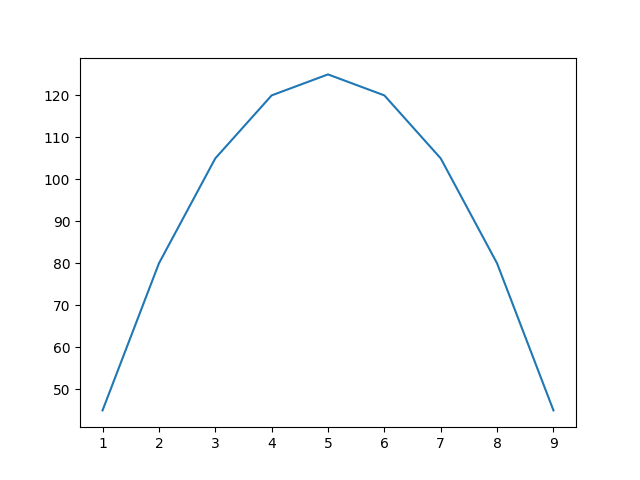
\includegraphics[width=\linewidth]{Figure_1.png}
  \caption{Drawing $\mybf{x}$. Multiplying a 9x9 second difference matrix by $\mybf{x}$ gives $\mybf{b} = (10, 10, \dots, 10)$ }
  \label{fig:kkk}
\end{figure}
\subsection*{section 3.3 Problem 36 (former section 3.4 - problem 36)}
My wrong answer:
Not necessarily. Let's take for example
\begin{align}
\begin{bmatrix}
1 & 1 \\
2 & 2 \\
\end{bmatrix}
\cdot \mybf{x} =
\begin{bmatrix}
1 \\
1 \\
\end{bmatrix}
\end{align}
vs.
\begin{align}
\begin{bmatrix}
1 & 1 \\
3 & 3 \\
\end{bmatrix}
\cdot \mybf{x} =
\begin{bmatrix}
1 \\
1 \\
\end{bmatrix}
\end{align}
Same solutions however A doesn't equal C
\end{document}